%%%%%%%%%%%%%%%%%%%%%%%%%%%%%%%%%%%%%%%%%%%%%%%%%%%%%%%%%%%%%%%%%%%%%%%%%%%%
%%                                                                        %%
%%                 Support de cours Programmation orientée objet                  %%
%%                                                                        %%
%%%%%%%%%%%%%%%%%%%%%%%%%%%%%%%%%%%%%%%%%%%%%%%%%%%%%%%%%%%%%%%%%%%%%%%%%%%%
%% Guillaume Moreau (EC Nantes)
%% création : 21/06/2004
%% dernière modification : 23/06/2004
%% historique :

%% il faut fixer l'URL base pour que les liens relatifs fonctionnent...
%% bizaremment fichu mais c'est comme ça.

\documentclass[allowframebreaks,xcolor=dvipsnames]{beamer}

\mode<presentation>
{
\usetheme{Antibes}
  % or ...

  %\setbeamercovered{transparent}
  % or whatever (possibly just delete it)
}
\useoutertheme{infolines}
\usecolortheme[named=RoyalBlue]{structure}

\uselanguage{french}
\languagepath{french}
\deftranslation[to=french]{definition}{définition}
\deftranslation[to=french]{Definition}{D\'efinition}
\deftranslation[to=french]{example}{exemple}
\deftranslation[to=french]{Example}{Exemple}
\deftranslation[to=french]{algorithm}{algorithme}
\deftranslation[to=french]{Algorithm}{Algorithme}

\setbeamertemplate{blocks}[rounded][shadow=true]
\setbeamertemplate{navigation symbols}{}
\setbeamertemplate{itemize item}[square]
\setbeamertemplate{itemize subitem}[triangle]

\usepackage[T1]{fontenc}
% or whatever

\usepackage[french]{babel}
% or whatever

\usepackage{tikz}
\usetikzlibrary{graphs}
\usetikzlibrary{graphdrawing.force}
\usetikzlibrary{arrows}
\usepackage{tikz-network}

%% pour afficher le plan à chaque début de section
%\AtBeginSection[]{
%  \begin{frame}{Plan}
%  \tiny \tableofcontents[currentsection, hideothersubsections]
%  \end{frame}
%}


%% tout ce qui est relatifs aux extraits de code
\usepackage{minted}
\newminted{python}{fontsize=\footnotesize}


\usepackage{myslides}

%% mes styles pour les graphes
\usepackage{graphstyle}

%\usepackage{times}
\usepackage[T1]{fontenc}
% Or whatever. Note that the encoding and the font should match. If T1
% does not look nice, try deleting the line with the fontenc.


\title[Option INFO / MADIS] % (optional, use only with long paper titles)
{Mathématiques discrètes : algorithmique des graphes}

\author[G. Moreau]{Guillaume Moreau\\
\texttt{guillaume.moreau@ec-nantes.fr}}
% - Use the \inst{?} command only if the authors have different
%   affiliation.

\institute[Ecole Centrale de Nantes] % (optional, but mostly needed)
{
  Ecole Centrale de Nantes
}

\date % (optional)
{Septembre 2020}

\subject{Théorie et algorithmique des graphes}


\definecolor{webgreen}{rgb}{0,.5,0}
\definecolor{webbrown}{rgb}{.6,0,0}
\definecolor{* }{rgb}{0,.5,0}
\definecolor{. }{rgb}{.6,0,0}

% option d'affiche de table des matières : http://mirror.unl.edu/ctan/macros/latex/contrib/beamer/doc/beameruserguide.pdf
% section 10.5

% Delete this, if you do not want the table of contents to pop up at
% the beginning of each subsection:
\AtBeginSection[]
{
   \begin{frame}
       \frametitle{Plan}
       \tableofcontents[sectionstyle=show/hide,subsectionstyle=show/show/hide,subsubsectionstyle=hide/hide]
   \end{frame}
}

\AtBeginSubsection[]
{
	\begin{frame}
		\frametitle{Plan}
		\tableofcontents[sectionstyle=show/hide,subsectionstyle=show/shaded/hide,subsubsectionstyle=show/show/hide]
	\end{frame}
}

\begin{document}

\begin{frame}
  \titlepage
\end{frame}

\begin{frame}[allowframebreaks]{Plan du cours}
  \tableofcontents[hideallsubsections]
  % You might wish to add the option [pausesections]
\end{frame}

% TODO ajouter un index


\section{Parcours de graphes}

% parcours de graphes 

\begin{frame}{Parcours de graphe}
\begin{itemize}
    \item Comment parcourir un graphe de façon exhaustive ?
    \item Explorer tous les sommets 
    \begin{itemize}
        \item En partant d'un sommet d'origine (ou plusieurs si le graphe n'est pas connexe / fortement connexe)
        \item En suivant uniquement les arcs qui sortent d'un sommet déjà exploré
        \item En construisant un historique de son parcours : notion d'arbre de \emph{parcours}
    \end{itemize}
    \item Routine de base en algorithmique des graphes 
\end{itemize}
\end{frame}

\begin{frame}{Comment ?}
    \begin{center}
        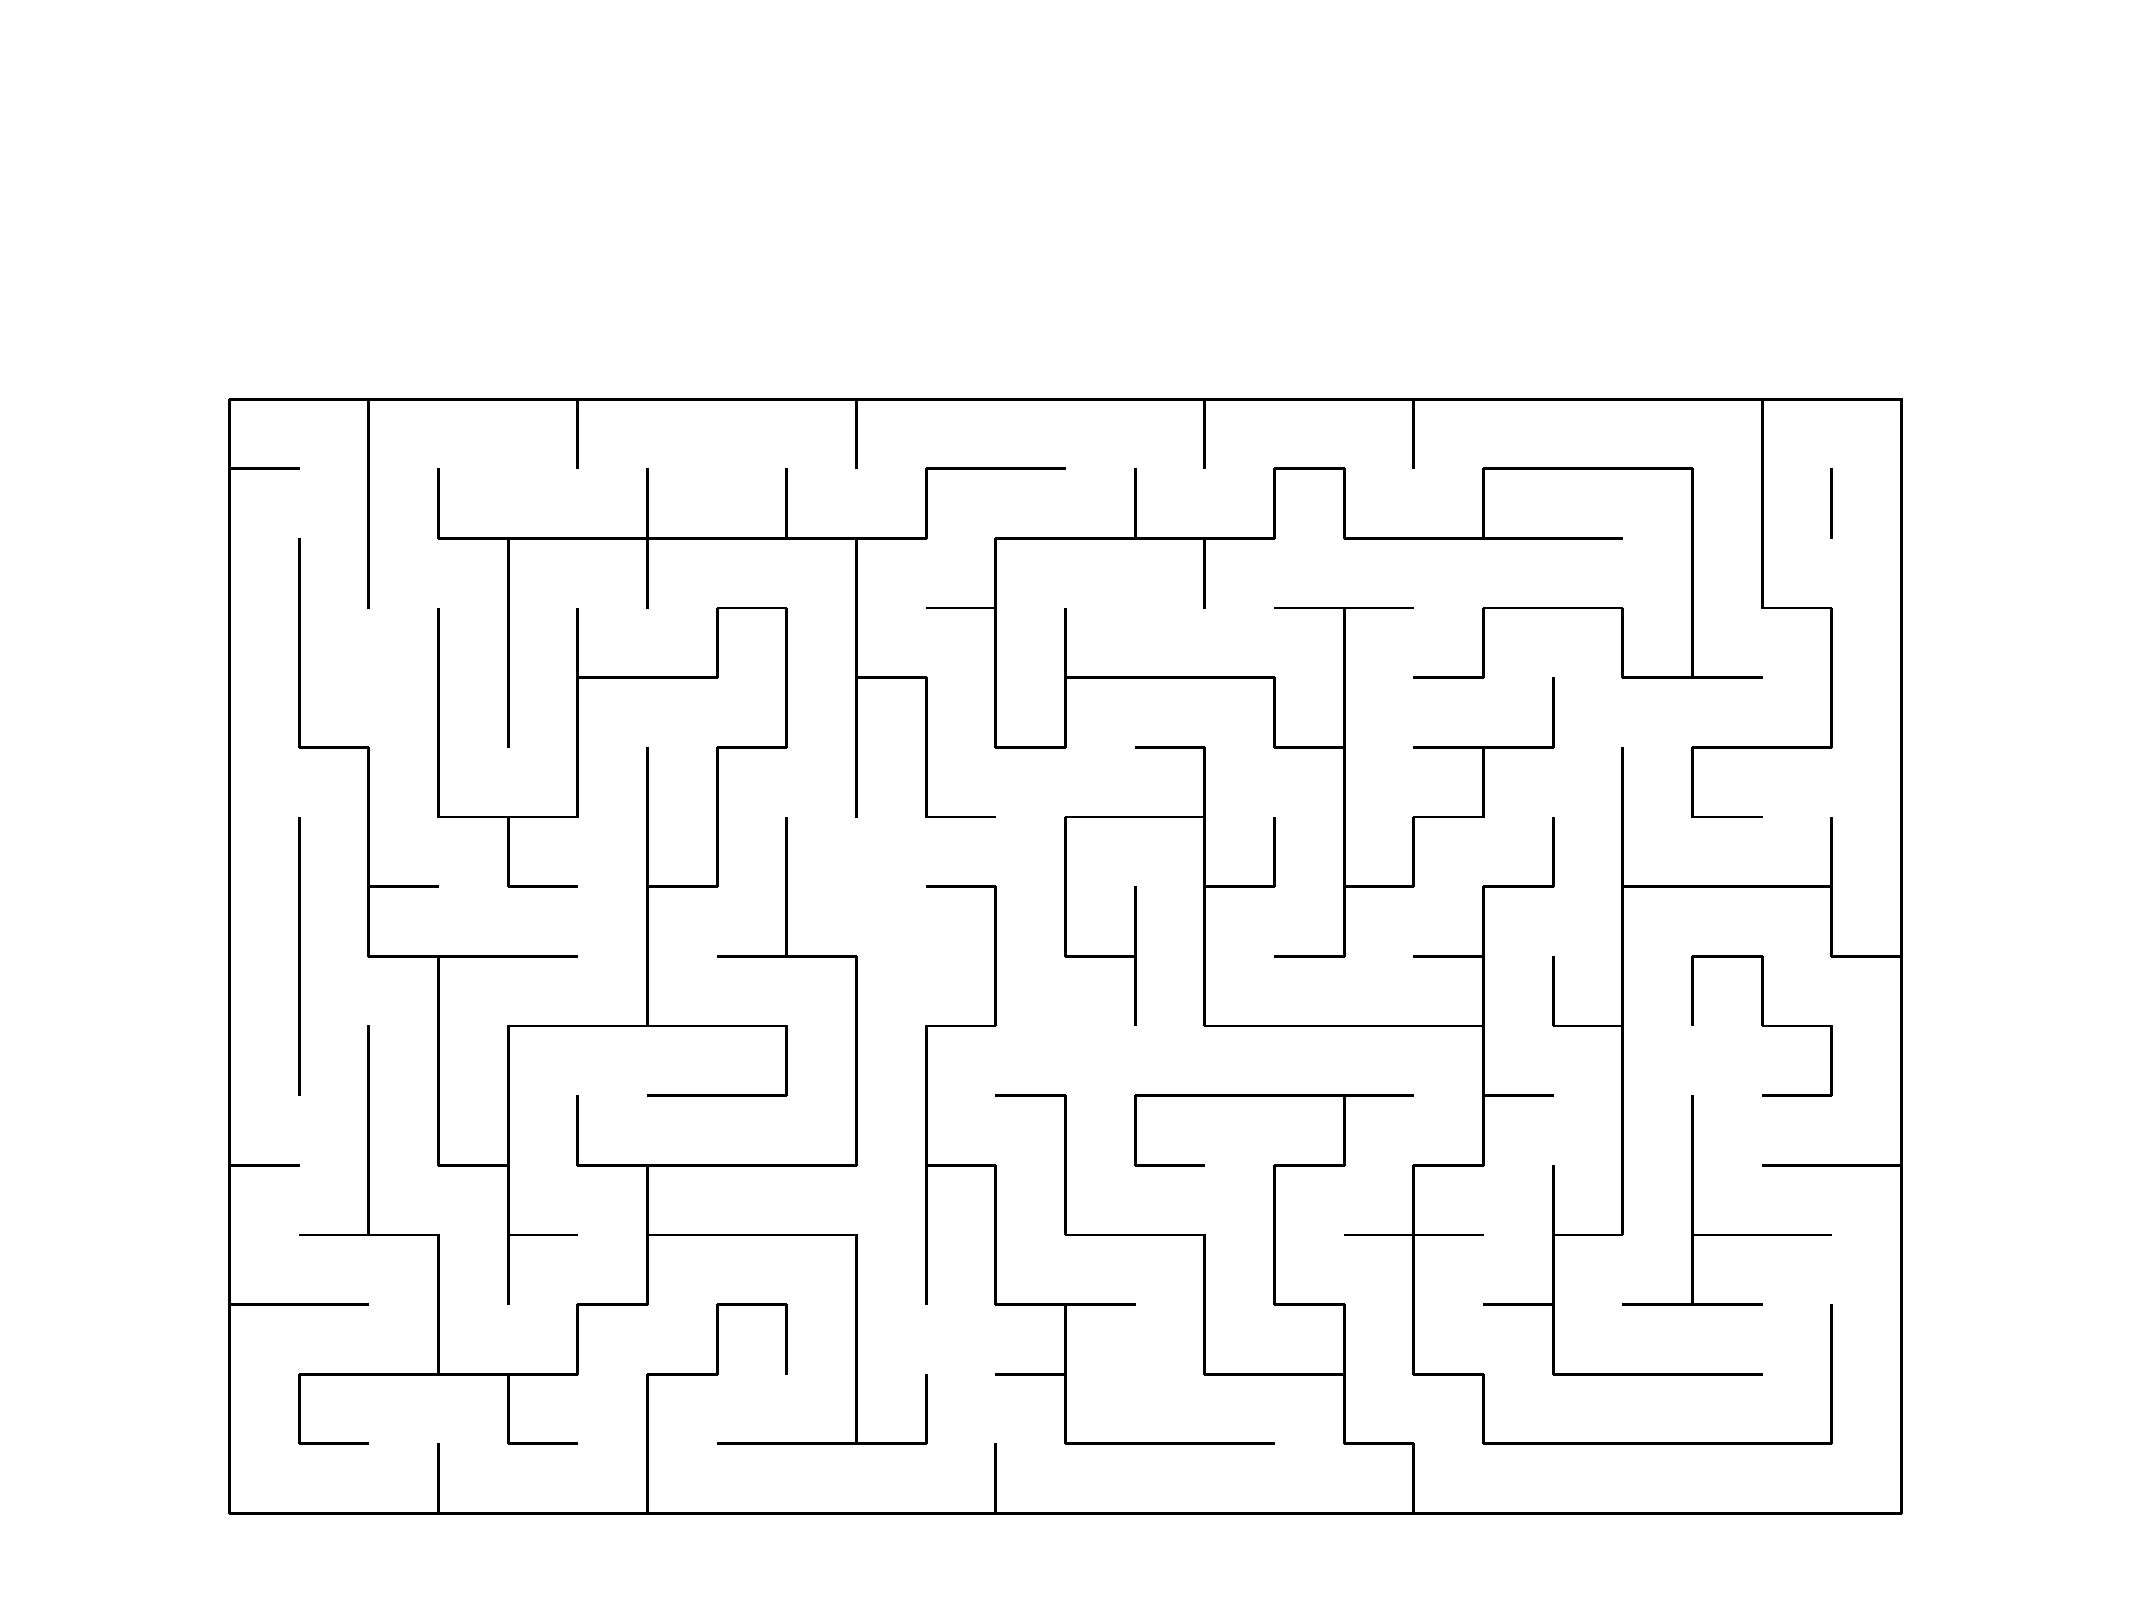
\includegraphics[width=.75\textwidth]{fig/labyrinthe.pdf}
    \end{center}
\end{frame}

\begin{frame}{Comment ?}
    \begin{center}
        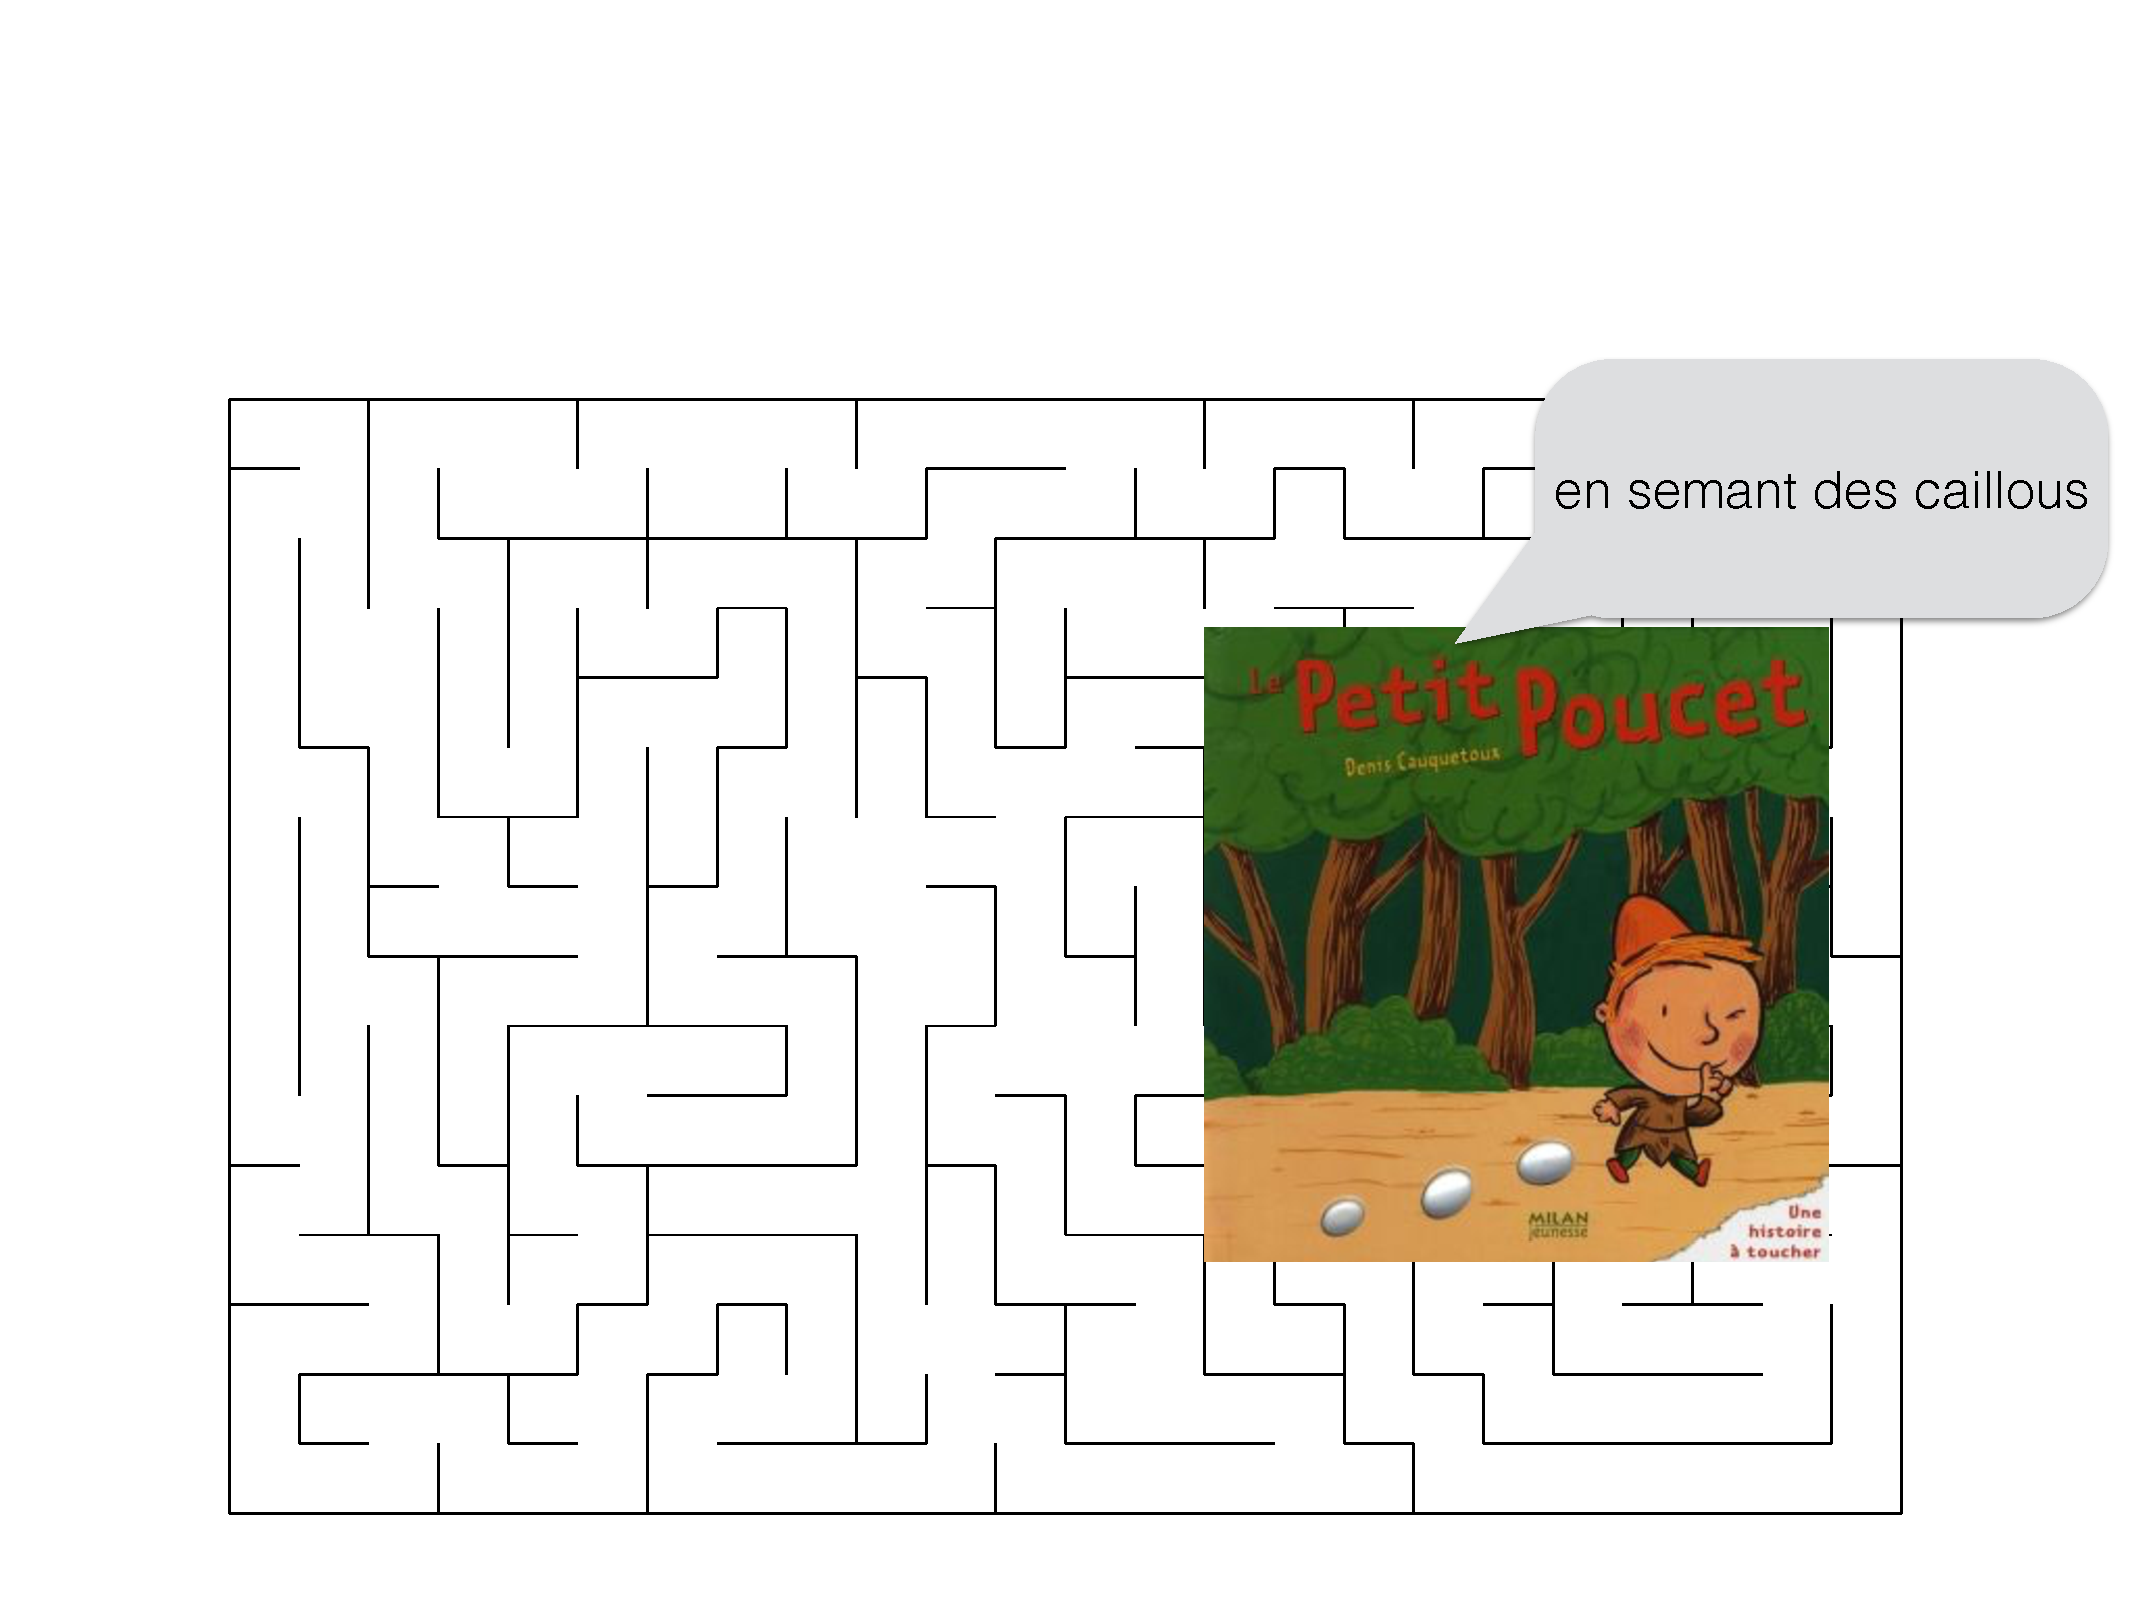
\includegraphics[width=.75\textwidth]{fig/labyrinthe-cailloux.pdf}
    \end{center}
\end{frame}

\begin{frame}{Comment ?}
    \begin{center}
        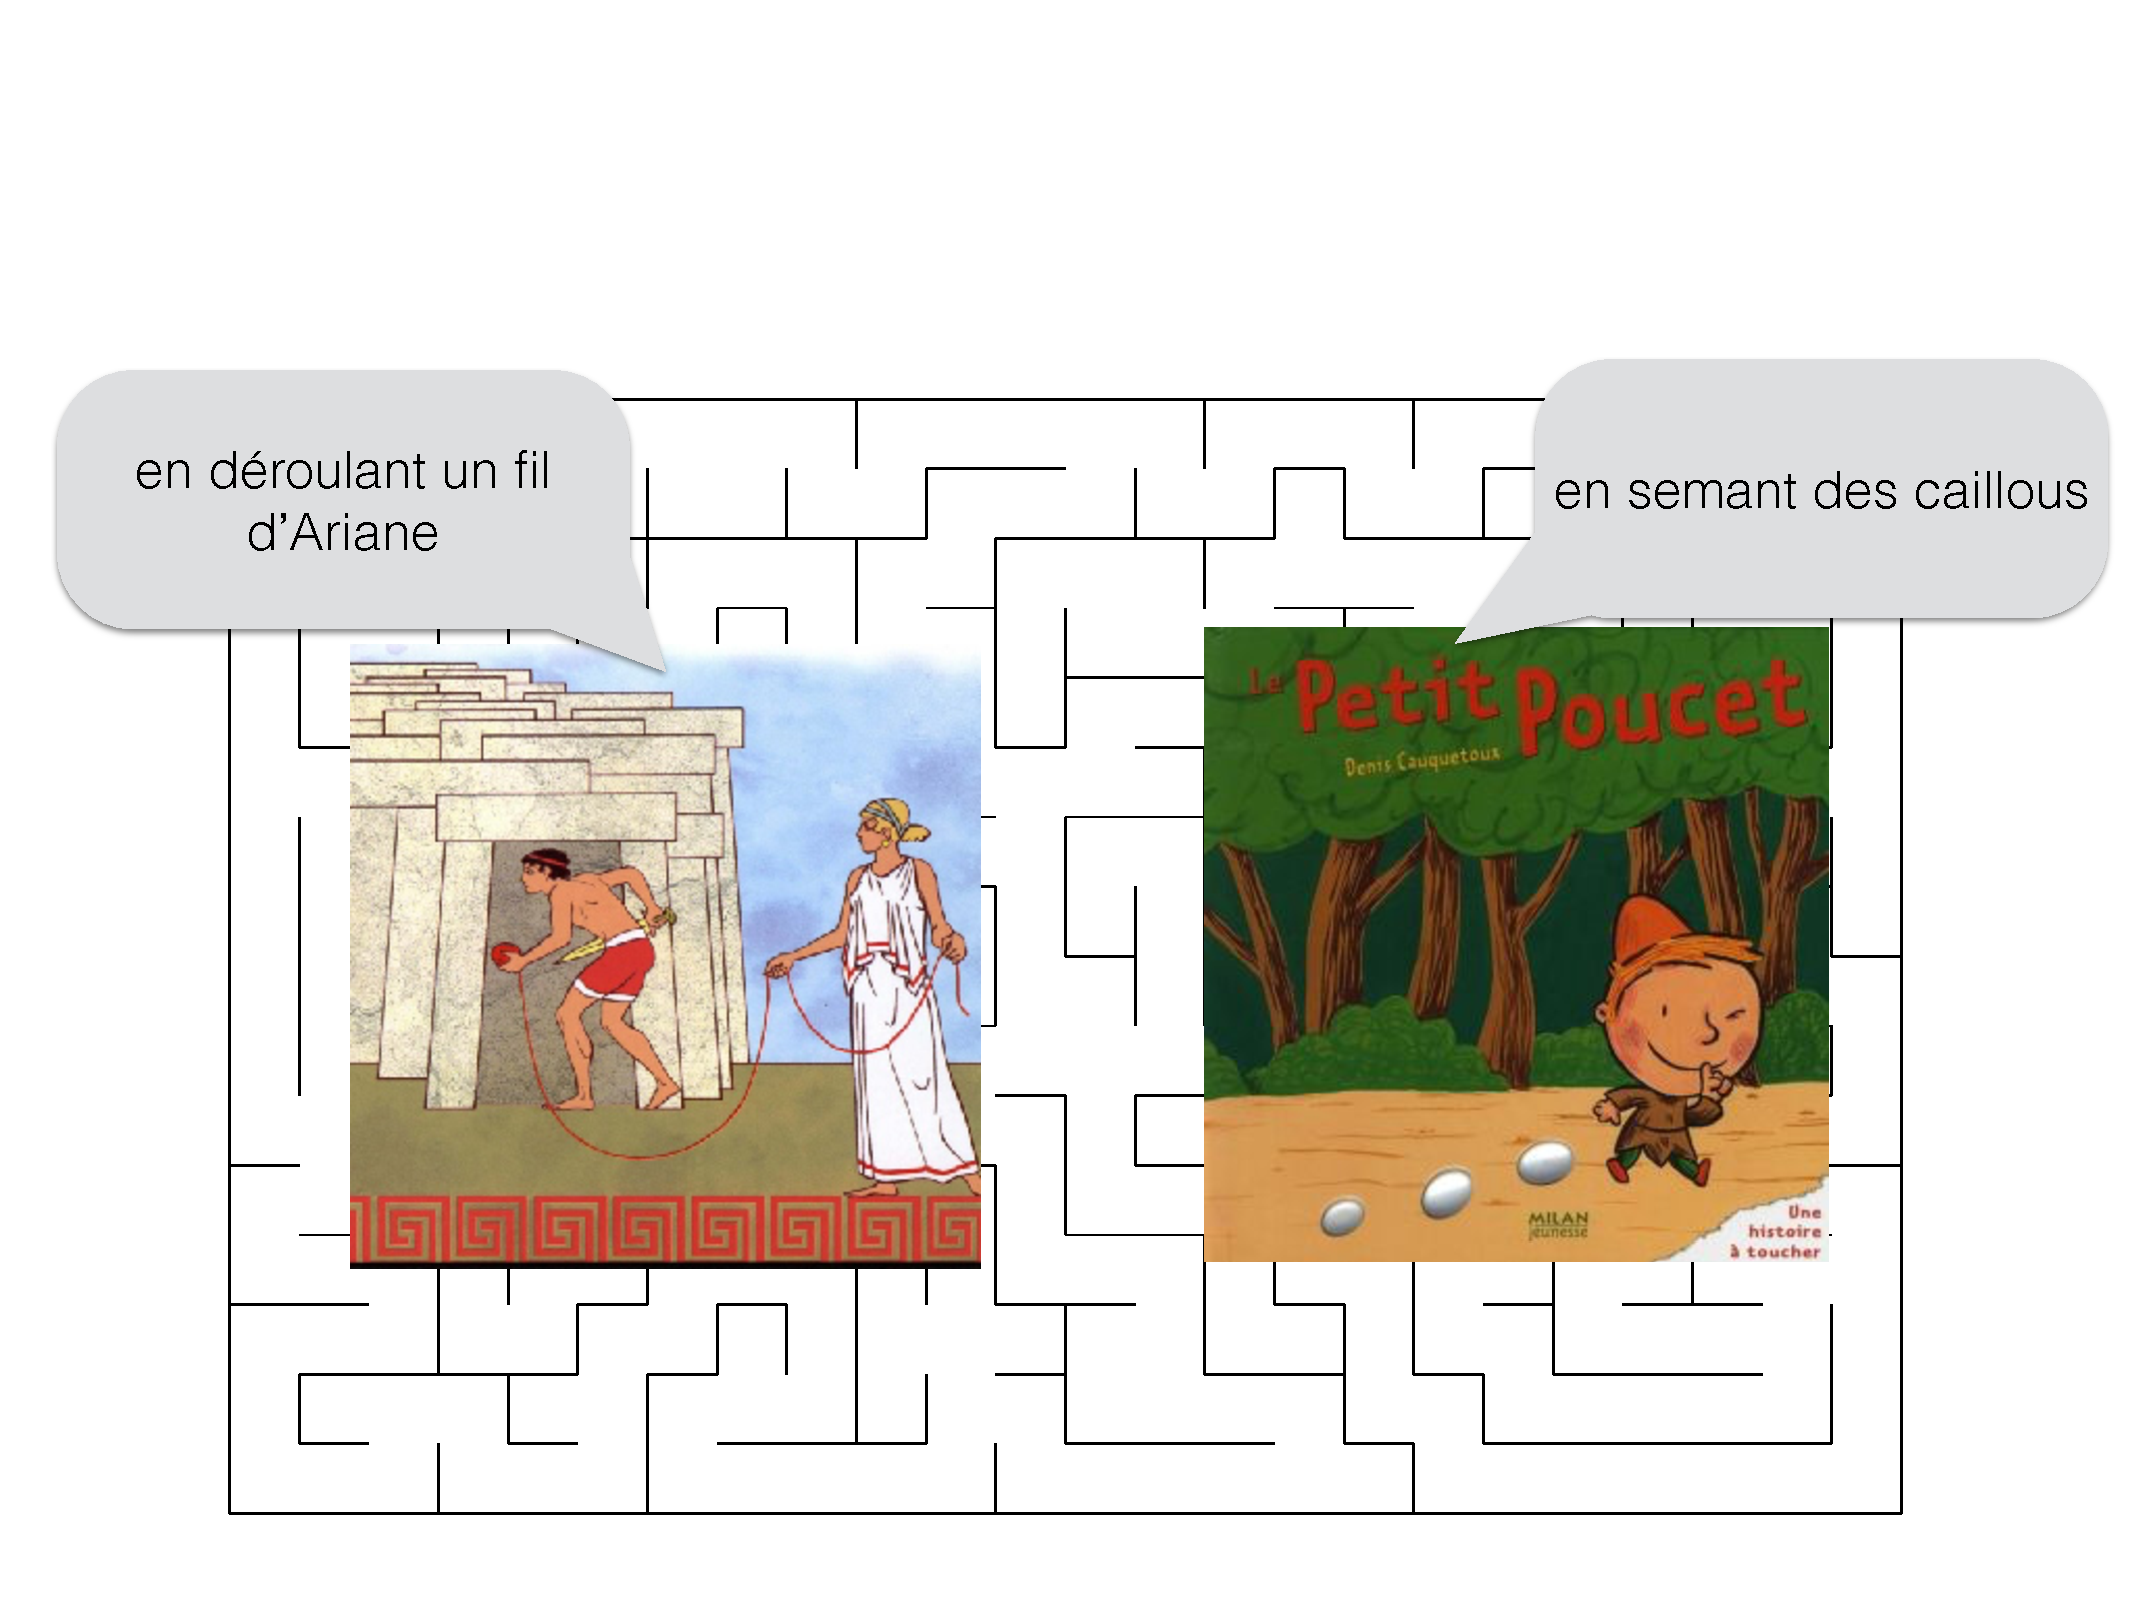
\includegraphics[width=.75\textwidth]{fig/labyrinthe-3.pdf}
    \end{center}
\end{frame}

\begin{frame}[fragile]
\frametitle{Parcours en profondeur}
    \begin{itemize}
        \item On utilise un tableau de booléens 
        \begin{itemize}
            \item \emph{vrai} si le sommet a été vu 
            \item \emph{faux} sinon 
        \end{itemize}
        \item on construit une fonction récursive \texttt{visite(i)} qui va explorer les sommets non vus à partir de $i$ ($i$ inclus)
    \end{itemize}
    
    % test
    \begin{algorithm}[H]
        \begin{algorithmic}[1]
            \Function{visite}{$i$ : sommet}
            \State vu[i] \gets true
            \For{$j \in Adj[i]$}
                \If{$vu[j] = false$}
                    \State visite(j)
                \EndIf
            \EndFor
            \EndFunction
         \end{algorithmic}
        \caption{Parcours en profondeur à partir d'un sommet}
        \label{alg:prof:visite}
        \end{algorithm}
\end{frame}



% ajouter la version avec les dates de visite ? pas sûr de l'intérêt ici...

\begin{frame}{Parcours en profondeur}
    \begin{itemize}
        \item Attention : l'algorithme n'est pas correct pour parcourir tout le graphe
        \item De fait, il ne fonctionne que si le graphe est connexe 
        \pause 
        \item On peut ajouter une boucle sur tous les sommets 
        \pause 
        \begin{algorithm}[H]
            \begin{algorithmic}[1]
                \State vu \gets [$false$,...,$false$]
                \For{$i \in S$}
                    \If{$vu[i] = false$}
                        \State visite(i)
                    \EndIf
                \EndFor
             \end{algorithmic}
            \caption{Parcours en profondeur}
            \label{alg:prof:alg}
            \end{algorithm}
        \pause 
        \item convention implicite : on parcourt les sommets et les adjacents en ordre croissant
    \end{itemize}
\end{frame}


\directlua{\detokenize{
    for i=0,6,1 do
        tex.sprint("\\begin{frame}{Exemple} \\input{genfig/pp-", i, ".tex} \\end{frame}")
    end
}}

\begin{frame}{Efficacité de l'algorithme}
    \begin{itemize}
        \item On marque $vu[i]$ une seule fois 
        \begin{itemize}
            \item Donc \texttt{visite(i)} termine toujours
            \item \texttt{visite(i)} n'est appelée qu'une seule fois par sommet
        \end{itemize}
        \item Le temps de calcul est dominé par les itérations de boucles
        \begin{itemize}
            \item La boucle principale s'exécute $n$ fois 
            \item La boucle secondaire s'exécute globalement $\sum_i | Adj[i] | = m$
        \end{itemize}
        \item La complexité pire cas est en $n+m$, donc linéaire
    \end{itemize}
\end{frame}

\begin{frame}{Forêts de parcours}
    \begin{itemize}
        \item Pendant un parcours en profondeur récursif, on peut créer une relation \emph{parent} qui mémorise pour chaque sommet $j$ 
        \begin{itemize}
            \item le sommet $i$ responsable de sa visite 
            \item $-1$ si le sommet $j$ est visité par la boucle principale 
        \end{itemize}
        \item Le graphe non-orienté associé à \emph{parent} (une arête entre $i$ et $j$ si $parent[i]=j$), forme une forêt de parcours 
    \end{itemize}
\end{frame}



\begin{frame}[fragile]
\frametitle{Algorithme}
    \begin{columns}
        \begin{column}{.5\textwidth}
            \begin{algorithmic}[1]
                \Function{visite}{$i$ : sommet}
                \State vu[i] \gets true
                \For{$j \in Adj[i]$}
                    \If{$vu[j] = false$}
                        \State \textcolor{blue}{parent[j] \gets i}
                        \State visite(j)
                    \EndIf
                \EndFor
                \EndFunction
            \end{algorithmic}
        \end{column}
        \begin{column}{.5\textwidth}
            \begin{algorithmic}[1]
                \State vu \gets [$false$,...,$false$]
                \State \textcolor{blue}{parent \gets [$-1$,...,$-1$]}
                \For{$i \in S$}
                    \If{$vu[i] = false$}
                    \State visite(i)
                    \EndIf
                \EndFor
                \end{algorithmic}            
        \end{column}
    \end{columns}    
\end{frame}


% ajouter un exemple sur les forets de parcours 
% cours David : 
%  un exemple jouet que je ne comprends pas 
%  un exemple de parcours sur un très grand graphe 

\begin{frame}{Exemples d'application}
    \begin{itemize}
        \item Les arbres (forêts) de parcours ont diverses applications
        \item Composantes connexes 
        \begin{itemize}
            \item Identification
            \item Parcours 
        \end{itemize}
        \item Graphe bipartis
    \end{itemize}
\end{frame}


\begin{frame}{Composantes connexes}
    \begin{itemize}
        \item Propriétés du parcours en profondeur
        \begin{itemize}
            \item \texttt{visite(i)} ne parcourt que les sommets accessibles depuis $i$ 
            \item elle parcourt tous ceux qui n'étaient pas marqués \texttt{vu} avant de démarrer la fonction 
        \end{itemize}
        \item Comptage du nombre de composantes connexes 
        \begin{itemize}
            \item Il suffit de rajouter un compteur dans la boucle principale 
            \item incrémenté à chaque appel à \texttt{visite(i)}
        \end{itemize}
    \end{itemize}
    \begin{center}
        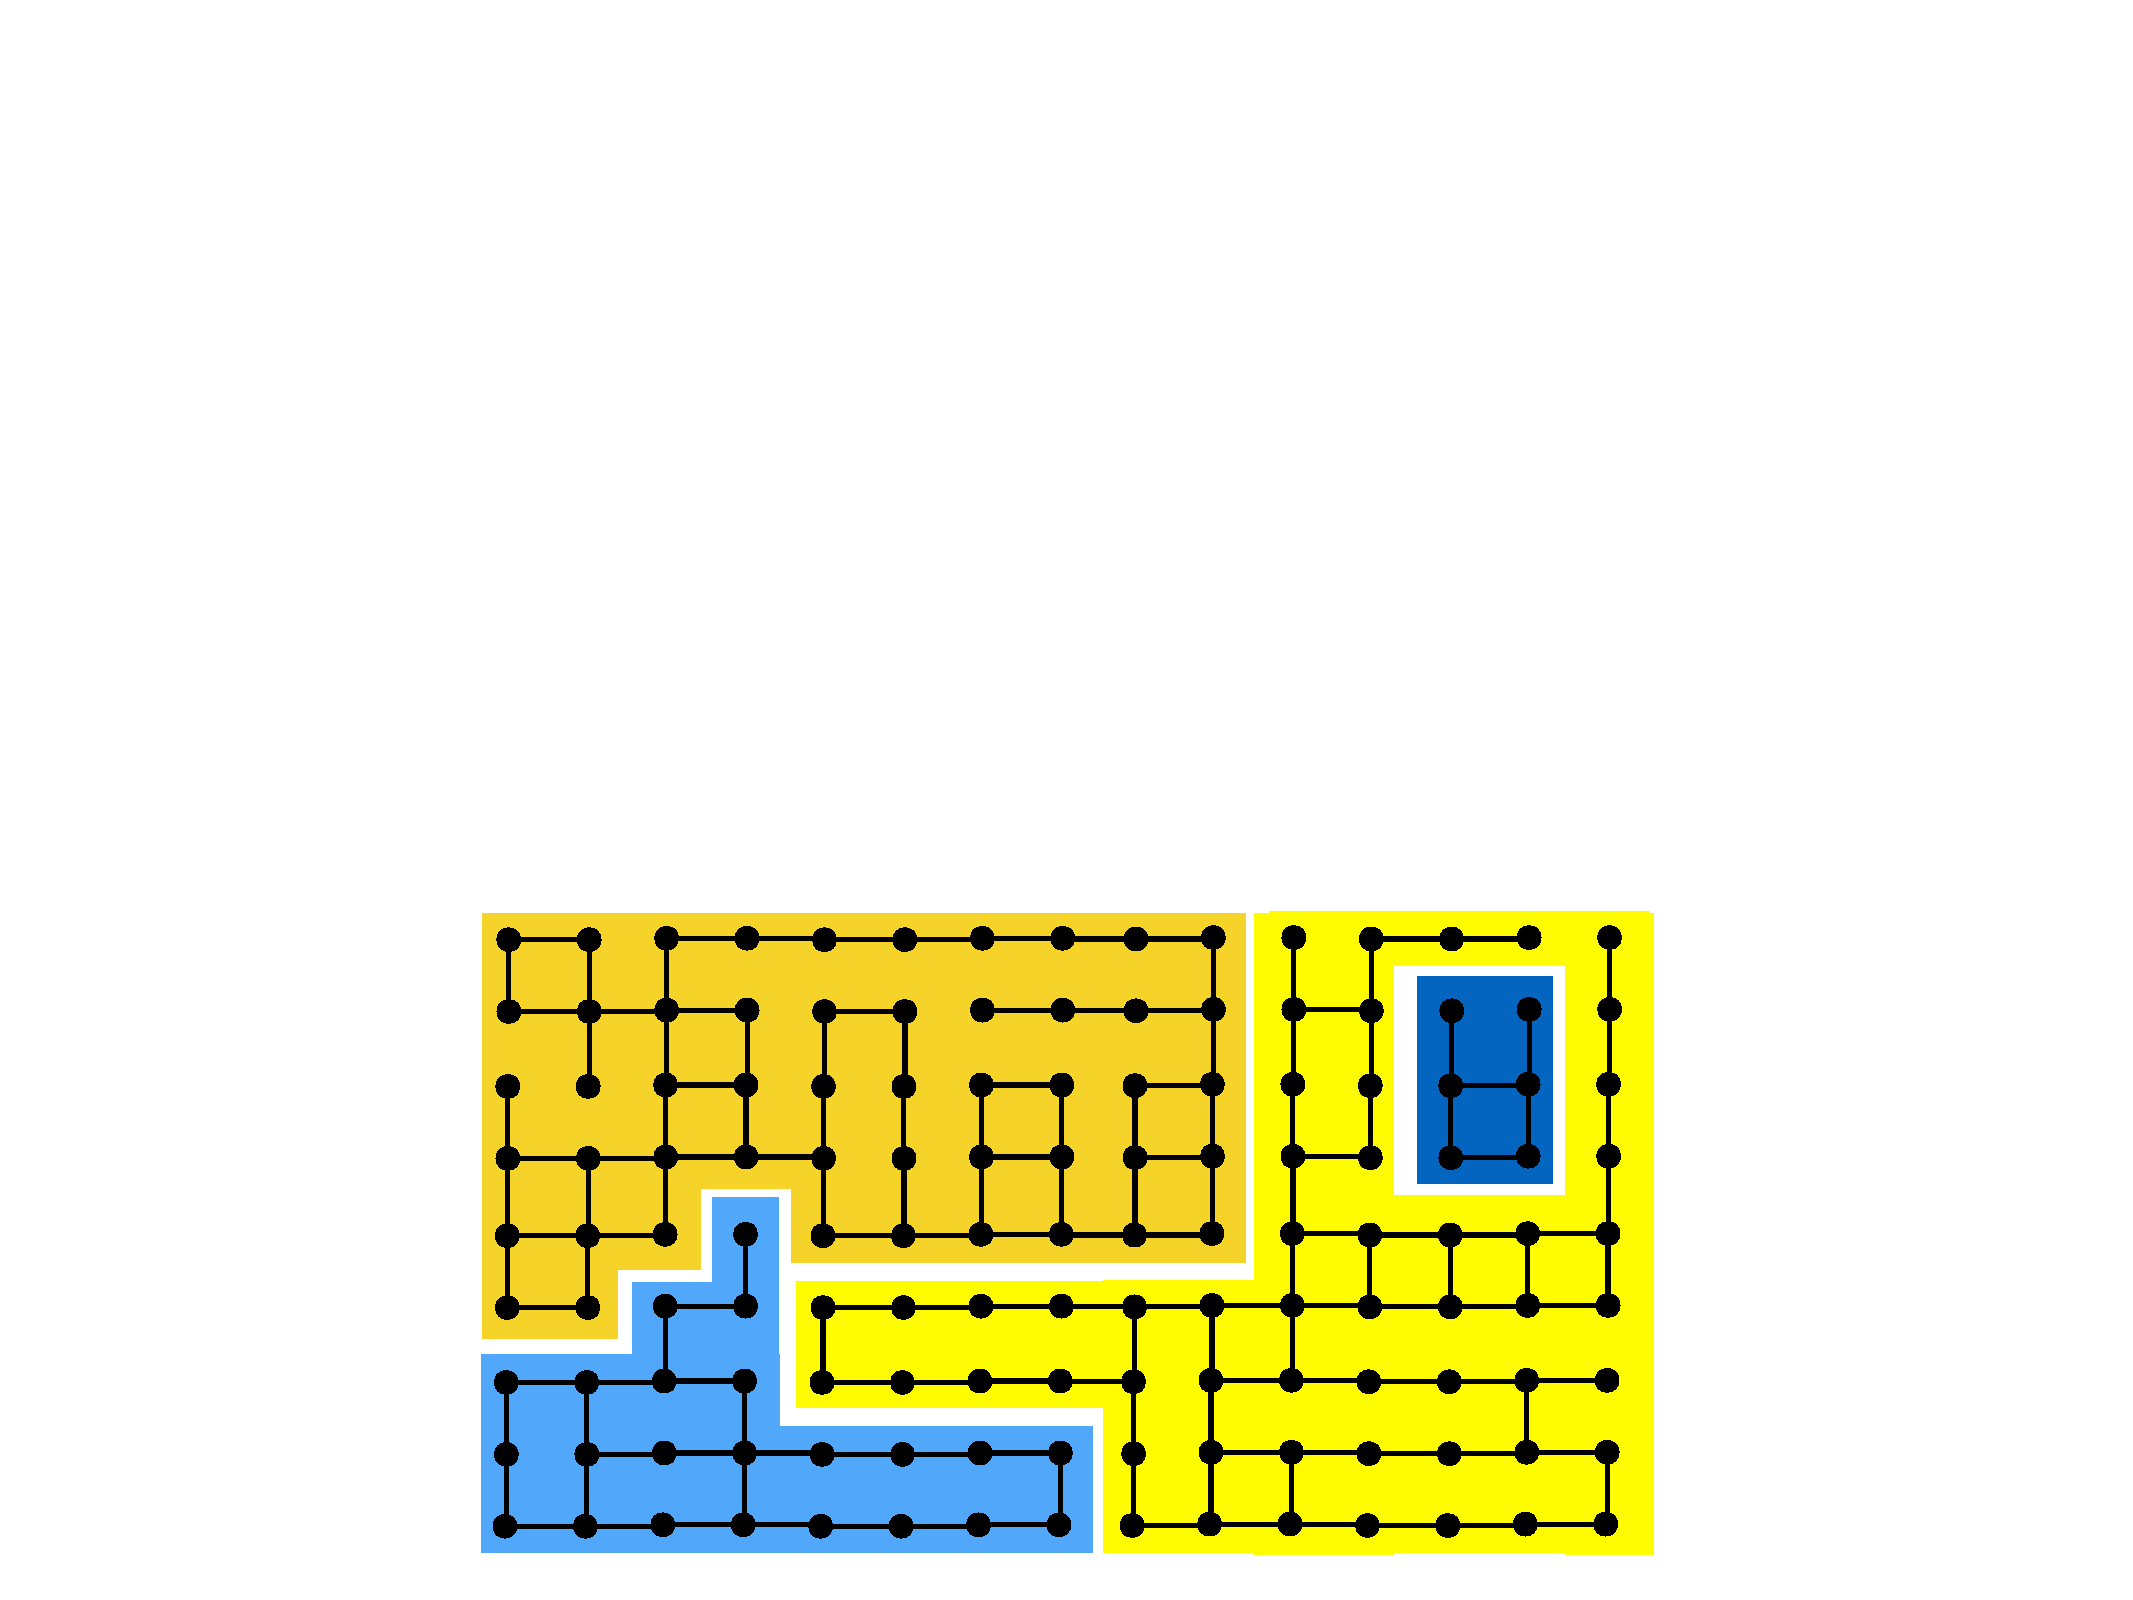
\includegraphics[width=.5\textwidth]{fig/cc.pdf}
    \end{center}
\end{frame}

\begin{frame}{Graphe biparti : plan de table}
    \begin{example}
        Pour un repas de famille, on doit réaliser un plan de table en tenant compte des inimitiés : les personnes qui ne s'aiment pas ne doivent pas se retrouver à la même table.        
    \end{example}
    \begin{center}
        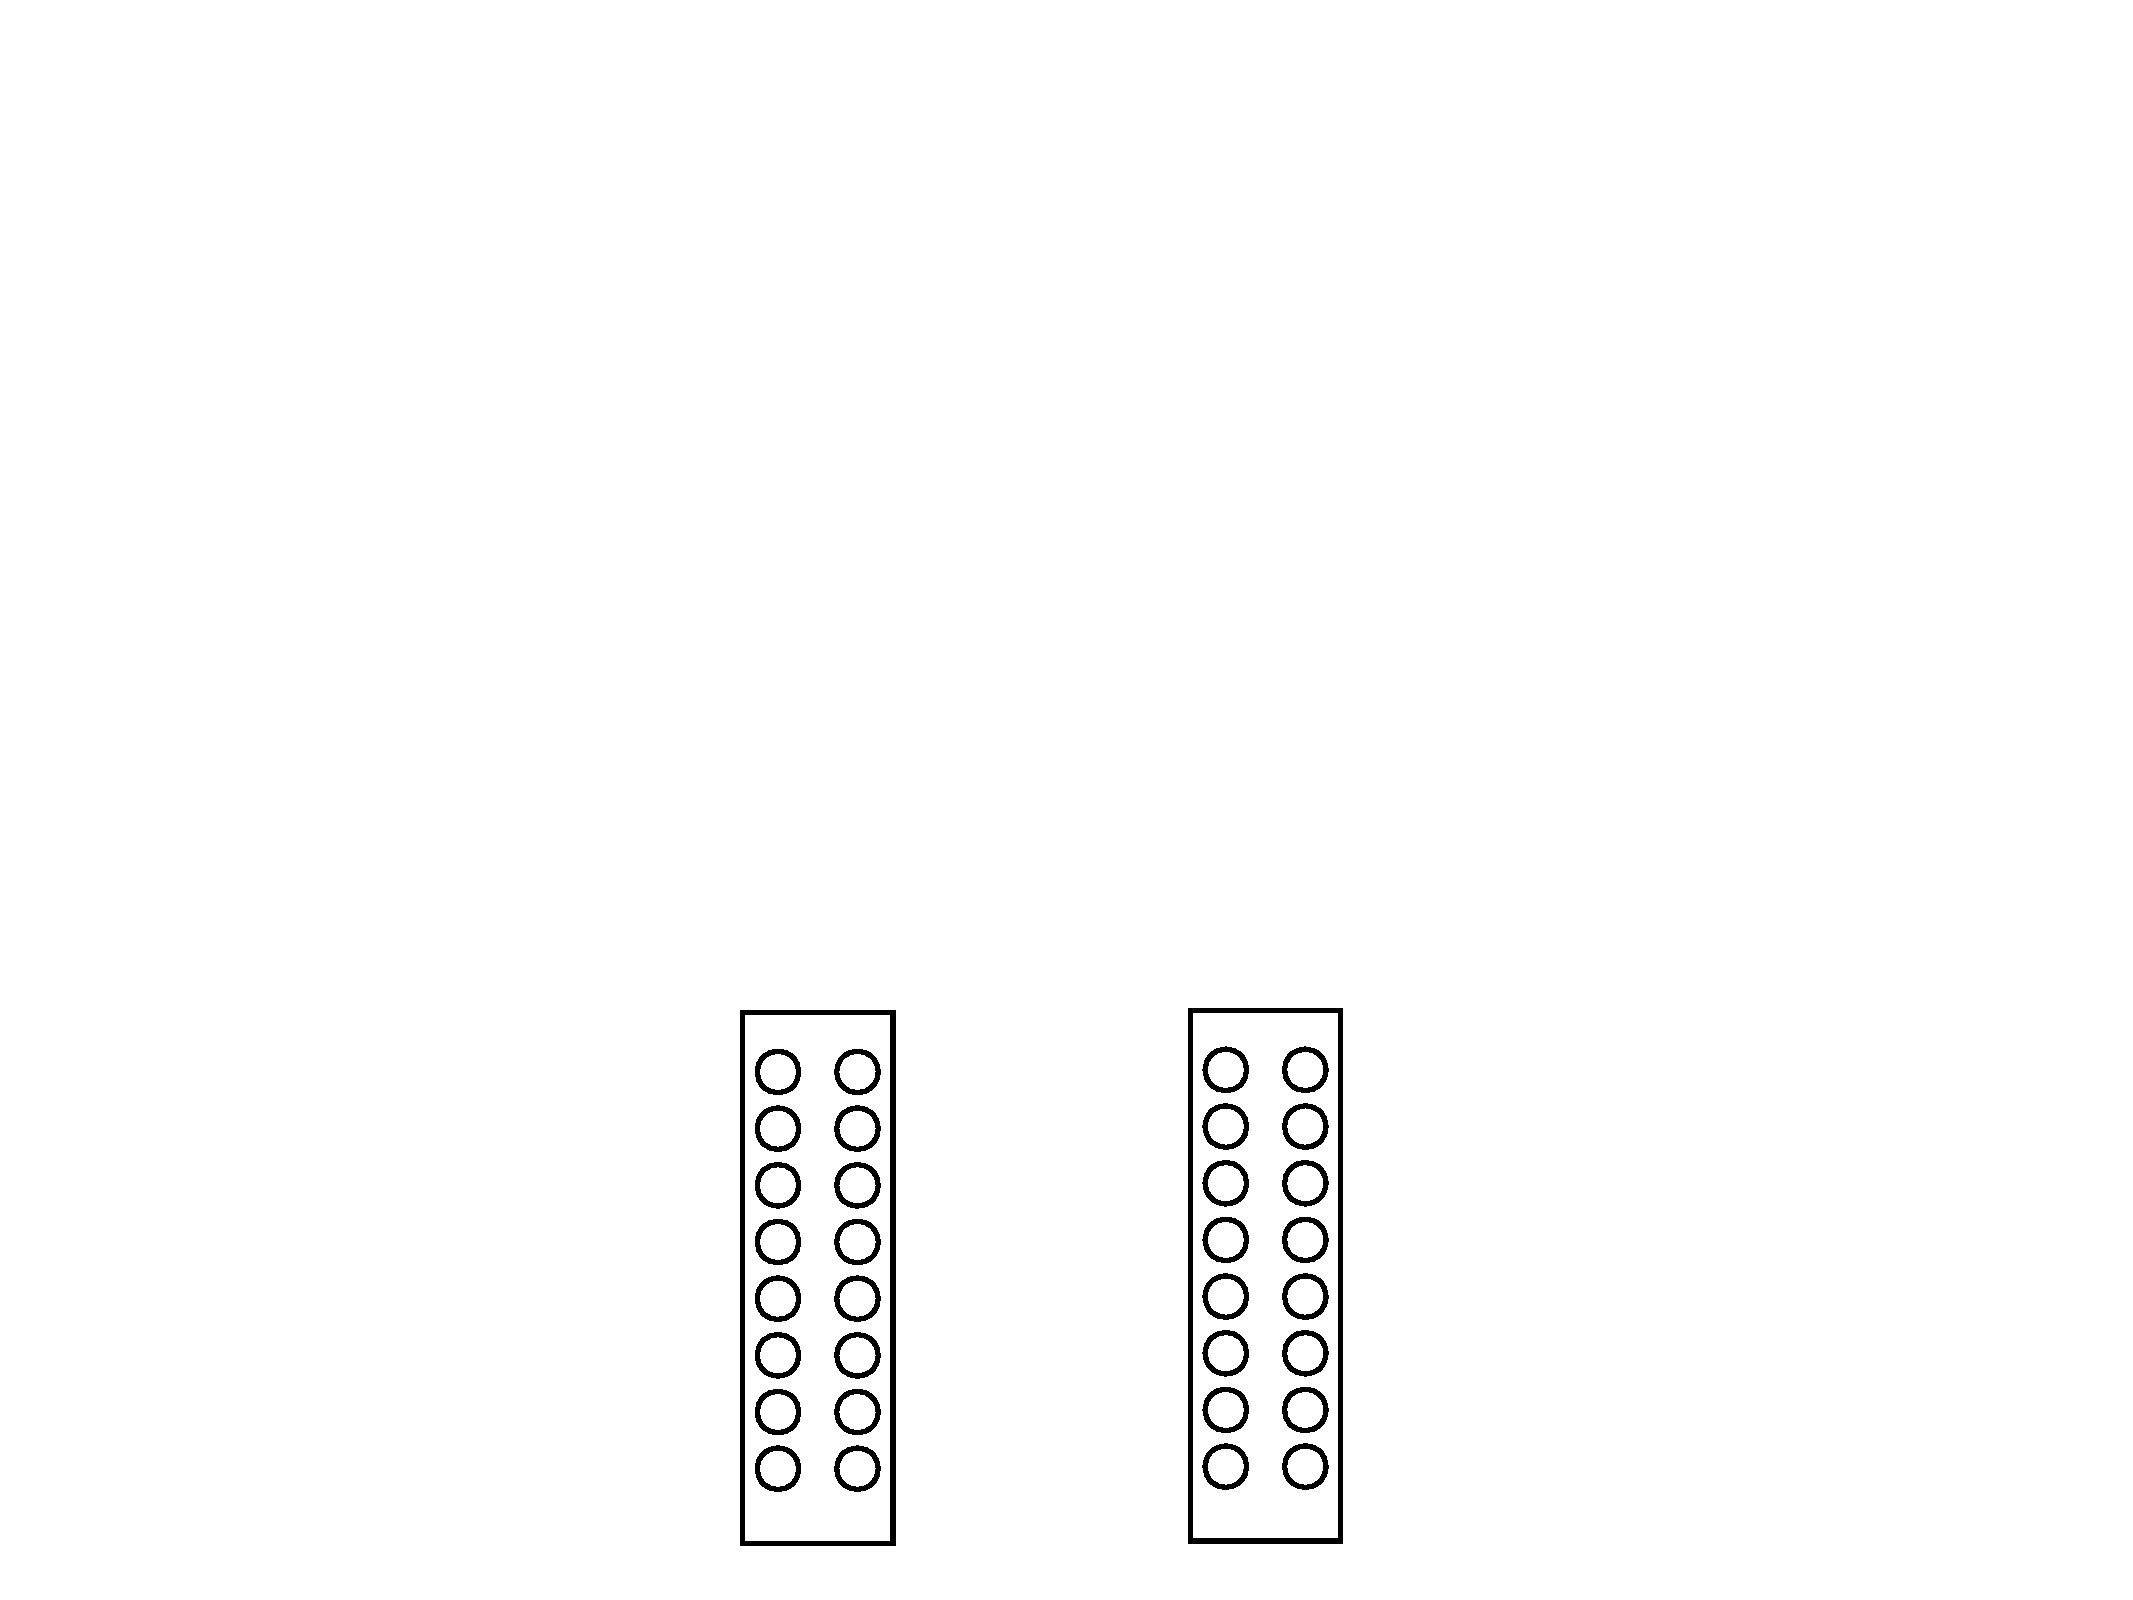
\includegraphics[width=.2\textwidth]{fig/plandetable.pdf}
    \end{center}
    \begin{definition}
        Un graphe non orienté est \emph{biparti} si l'ensemble des sommets peut être séparé en deux ensembles disjoints $S_1$ et $S_2$ tel que chaque arête du graphe relie un sommet de $S_1$ à un sommet de $S_2$ 
    \end{definition}
\end{frame}

\begin{frame}{Exemple}
    \begin{center}
    \begin{tikzpicture}
        \tikzstyle{sommet}=[circle,draw,fill=black]
        \node[sommet] (1) at (1,0) {};
        \node[sommet] (2) at (1,-1) {};
        \node[sommet] (3) at (1,-2) {};
        \node[sommet] (4) at (1,-3) {};
        \node[sommet] (5) at (2,0) {};
        \node[sommet] (6) at (2,-1) {};
        \node[sommet] (7) at (2,-2) {};
        \node[sommet] (8) at (2,-3) {};
        \node[sommet] (9) at (3,0) {};
        \node[sommet] (10) at (3,-1) {};
        \node[sommet] (11) at (3,-2) {};
        \node[sommet] (12) at (3,-3) {};
        \node[sommet] (13) at (4,0) {};
        \node[sommet] (14) at (4,-1) {};
        \node[sommet] (15) at (4,-2) {};
        \node[sommet] (16) at (4,-3) {};
        \node[sommet] (17) at (5,0) {};
        \node[sommet] (18) at (5,-1) {};
        \node[sommet] (19) at (5,-2) {};
        \node[sommet] (20) at (5,-3) {};
        \node[sommet] (21) at (6,0) {};
        \node[sommet] (22) at (6,-1) {};
        \node[sommet] (23) at (6,-2) {};
        \node[sommet] (24) at (6,-3) {};
        \draw (1) -- (2) -- (3) -- (4);
        \draw (6) -- (7) -- (8);
        \draw (9) -- (10) -- (11);
        \draw (13) -- (14);
        \draw (15) -- (16);
        \draw (17) -- (18) -- (19);
        \draw (21) -- (22) -- (23);
        \draw (2) -- (6) -- (10) -- (14) -- (18);
        \draw (3) -- (7) -- (11);
        \draw (19) -- (23);
        \draw (4) -- (8);
        \draw (12) -- (16);
        \draw (20) -- (24); 
    \end{tikzpicture}
\end{center}
\end{frame}

\begin{frame}{Exemple}
    \begin{center}
    \begin{tikzpicture}
    \tikzstyle{sommetA}=[circle,draw,fill=blue]
    \tikzstyle{sommetB}=[circle,draw,fill=red]
    \node[sommetA] (1) at (1,0) {};
    \node[sommetB] (2) at (1,-1) {};
    \node[sommetA] (3) at (1,-2) {};
    \node[sommetB] (4) at (1,-3) {};
    \node[sommetA] (5) at (2,0) {};
    \node[sommetA] (6) at (2,-1) {};
    \node[sommetB] (7) at (2,-2) {};
    \node[sommetA] (8) at (2,-3) {};
    \node[sommetA] (9) at (3,0) {};
    \node[sommetB] (10) at (3,-1) {};
    \node[sommetA] (11) at (3,-2) {};
    \node[sommetA] (12) at (3,-3) {};
    \node[sommetB] (13) at (4,0) {};
    \node[sommetA] (14) at (4,-1) {};
    \node[sommetA] (15) at (4,-2) {};
    \node[sommetB] (16) at (4,-3) {};
    \node[sommetA] (17) at (5,0) {};
    \node[sommetB] (18) at (5,-1) {};
    \node[sommetA] (19) at (5,-2) {};
    \node[sommetB] (20) at (5,-3) {};
    \node[sommetB] (21) at (6,0) {};
    \node[sommetA] (22) at (6,-1) {};
    \node[sommetB] (23) at (6,-2) {};
    \node[sommetA] (24) at (6,-3) {};
    \draw (1) -- (2) -- (3) -- (4);
    \draw (6) -- (7) -- (8);
    \draw (9) -- (10) -- (11);
    \draw (13) -- (14);
    \draw (15) -- (16);
    \draw (17) -- (18) -- (19);
    \draw (21) -- (22) -- (23);
    \draw (2) -- (6) -- (10) -- (14) -- (18);
    \draw (3) -- (7) -- (11);
    \draw (19) -- (23);
    \draw (4) -- (8);
    \draw (12) -- (16);
    \draw (20) -- (24); 
\end{tikzpicture}
\end{center}
\end{frame}

\begin{frame}[fragile]
\frametitle{Algorithme : principe}

\begin{itemize}
    \item Pendant un parcours en profondeur, on associe une couleur (0 ou 1) à chaque sommet en s'assurant que deux sommets adjacents n'ont pas la même couleur 
    \item Si l'algorithme termine sans erreur, on a examiné chaque arête et attribué des couleurs cohérentes à chaque sommet : le graphe est biparti 
    \item Sinon, le coloriage est impossible et l'algorithme s'arrête avant la fin 
\end{itemize}
\end{frame}

    \begin{frame}[fragile]
        \frametitle{Algorithme}
            \begin{columns}
                \begin{column}{.55\textwidth}
                    \begin{algorithmic}
                    \Function{visite}{$i$ : sommet,$c$ : int}
                    \State vu[i] \gets true
                    \State couleur[i] \gets $c$
                    \For{$j \in Adj[i]$}
                        \If{$vu[j] = false$}
                            \State visite(j,1-$c$)
                        \ElsIf{couleur[j] = $c$} 
                                \State STOP("pas biparti")
                        \EndIf
                    \EndFor
                    \EndFunction
                                    \end{algorithmic}
                \end{column}
                \begin{column}{.45\textwidth}
                    \begin{algorithmic}
                        \State vu \gets [$false$,...,$false$]
                        \State couleur \gets $[-1,...,-1]$
                        \For{$i \in S$}
                            \If{$vu[i] = false$}
                                \State visite(i)
                            \EndIf
                        \EndFor
                    \end{algorithmic}            
                \end{column}
            \end{columns}    
        \end{frame}
        
\begin{frame}{k-coloration}
\begin{definition}
    Un graphe non-orienté est \emph{$k$-coloriable} si on peut colorier chaque sommet avec une couleur comprise entre $1$ et $k$, de telle façon que deux sommets adjacents aient des couleurs distinctes
\end{definition}
\begin{itemize}
    \item Remarques 
    \begin{itemize}
        \item Un graphe biparti est un graphe $2$-coloriable 
        \item L'algorithme de $2$-coloration vu précédemment est linéaire, ce n'est pas généralisable malheureusement
        \item De fait, pour $k>2$, le problème de déterminer si un graphe est $k$-coloriable est NP-complet  
    \end{itemize}
\end{itemize}
\end{frame}

% parcours en profondeur (version non récursive) 

\begin{frame}{Dérécursification}

\begin{itemize}
    \item Tout programme récursif peut être transformé en un programme équivalent non récursif, en s'aidant d'une \emph{pile} 
    \begin{itemize}
        \item cela peut avoir un intérêt pour l'efficacité (peu probable)
        \item certains compilateurs savent le faire automatiquement (HS ici) 
        \item dans certains cas, c'est plus facile à comprendre 
    \end{itemize}
\end{itemize}
\end{frame}

\begin{frame}[fragile]
    \frametitle{Algorithme de parcours en profondeur itératif}
        \begin{columns}
            \begin{column}{.55\textwidth}
                \begin{algorithmic}
                    \Function{visite}{$i$ : sommet}
                    \State P \gets empty() 
                    \State vi[i] \ gets true 
                    \State push(P,i) 
                    \While{!empty(P)}
                        \State k \gets pop(P)
                        \For{$j \in Adj[k]$}
                            \If{!vu[j]} 
                            \State vu[k] \gets true 
                            \State push(P,j
                            \EndIf
                        \EndFor
                    \EndWhile
                    \EndFunction
                \end{algorithmic}
            \end{column}
            \begin{column}{.45\textwidth}
                \begin{algorithmic}
                    \State vu \gets [$false$,...,$false$]
                    \For{$i \in S$}
                        \If{$vu[i] = false$}
                            \State visite(i)
                        \EndIf
                    \EndFor
                \end{algorithmic}            
            \end{column}
        \end{columns}    
    \end{frame}



\section{Calcul de la fermeture transitive}

\begin{frame}{Calcul de la fermeture transitive dans un graphe \emph{creux}}
    \begin{columns}
    \begin{column}{0.5\textwidth}
        \begin{algorithmic}
            \Function{visite}{l,i}
            \State $A^*[l,i]$ \gets True 
            \For{$j \in \Gamma(i)$} 
            \If{non $A^*[l,j]$}  
                \State visite(l,j)
            \EndIf
            \EndFor
            \EndFunction
        \end{algorithmic}
    \end{column}
    \begin{column}{0.5\textwidth}
        \begin{algorithmic}
            \Function{fermeture transitive}{}
                \State $A^*$ = [[False,False],...[False,False]]
                \For{$i \in S$} 
                    \State visite(i,i)
                \EndFor \\
            \Return $A^*$
            \EndFunction
        \end{algorithmic}
    \end{column}
    \end{columns}
    \end{frame}
    
    \begin{frame}{Exemple}
    \begin{center}
        \input{genfig/ft0}
    \end{center}
    \end{frame}
    
    \begin{frame}{Exemple : fermeture réflexo-transitive}
    \begin{center}
        \input{genfig/ft1}
    \end{center}
        \end{frame}
    
    \begin{frame}{Calcul de la fermeture transitive}
    \begin{itemize}
        \item La calcul se fait en ${\cal O}(nm)$ avec $n$ parcours en profondeur
        \item En pratique, $A*$ est plutôt dense... On peut faire le calcul de façon matricielle
        \item cf. algorithme de Floyd-Warshall en TD 
    \end{itemize}
    \end{frame}
    

\section{Calcul des composantes fortement connexes}

% calcul des composantes fortement connexes 

\begin{frame}{Calcul des composantes fortements connexes : un peu d'histoire}

\begin{itemize}
    \item Années 60 : un problème classique 
    \begin{itemize}
        \item mais sans solution efficace (polynomiale)
        \item la complexité du problème n'est pas connue 
    \end{itemize}
    \item 1972 : algorithme linéaire proposé par Trojan 
    \begin{itemize}
        \item simple modification du parcours en profondeur 
        \item difficile à comprendre 
    \end{itemize}
    \item années 80 : algorithme linéaire de Kosajaru 
    \begin{itemize}
        \item plus simple à comprendre (2 parcours)
        \item la légende dit qu'il avait oublié ses notes de cours et qu'il a inventé l'algorithme en préparant son cours 
    \end{itemize}
\end{itemize}
\end{frame}

\begin{frame}{Notion de graphe inverse}
\begin{definition}
    Le graphe \emph{inverse} d'un graphe $G=(S,A)$ est le graphe $G'=(S,A')$ possédant les mêmes sommets mais possédant un arc $(i,j) \in A'$ si et seulement si $(j,i) \in A$    
\end{definition}

\begin{example}
    \begin{tikzpicture}
        \node[lettre] (1) at (0,0)  {1};
        \node[lettre] (2) at (0,-1) {2};
        \node[lettre] (3) at (1,-1) {3};
        \node[lettre] (4) at (1,0) {4};
        \node[lettre] (5) at (2,0) {5};
        \node[lettre] (6) at (2,-1) {6}; 
        \draw[edge] (1) -> (4);
        \draw[edge] (1) -> (2) -> (4);
        \draw[edge] (2) -> (3);
        \draw[edge] (6) -> (5);
        \draw[edge] (4.260) -> (3.100);
        \draw[edge] (3.800) -> (4.280);
        \node (l) at (4.5,0) { et son graphe inverse};
    \end{tikzpicture}        
    \begin{tikzpicture}
        \node[lettre] (1) at (0,0)  {1};
        \node[lettre] (2) at (0,-1) {2};
        \node[lettre] (3) at (1,-1) {3};
        \node[lettre] (4) at (1,0) {4};
        \node[lettre] (5) at (2,0) {5};
        \node[lettre] (6) at (2,-1) {6}; 
        \draw[edge] (4) -> (1);
        \draw[edge] (4) -> (2) -> (1);
        \draw[edge] (3) -> (2);
        \draw[edge] (5) -> (6);
        \draw[edge] (4.260) -> (3.100);
        \draw[edge] (3.800) -> (4.280);
    \end{tikzpicture}        
\end{example}

\begin{block}{Propriété}
    Les composantes fortement connexes d'un graphe sont identiques à celles de son graphe inverse
\end{block}

\end{frame}

\begin{frame}{Algorithme de Kosaraju : principe}

\begin{enumerate}
    \item Parcours en profondeur de $G$ pour retenir un ordre suffixe
    \begin{itemize}
        \item i.e. quand on visite $b$ depuis $a$, on note $b$, $a$
    \end{itemize}
    \item Calcul de $G'$ l'inverse de $G$
    \item Parcours en profondeur sur $G'$ mais avec modification de la boucle principale : on prend la boucle principale par l'inverse de l'ordre suffixe établi à la première étape
    \item Les composantes fortement connexes sont les arbres de la forêt du second parcours
\end{enumerate}

\end{frame}

\begin{frame}[fragile]
    \frametitle{Algorithme de Kosaraju (partie 1)}
        \begin{columns}
            \begin{column}{.5\textwidth}
                \begin{algorithmic}[1]
                    \Function{visite}{$i$ : sommet}
                    \State vu[i] \gets true
                    \For{$j \in Adj[i]$}
                        \If{$vu[j] = false$}
                            \State visite(j)
                        \EndIf
                    \EndFor
                    \State \textcolor{blue}{os.add(i)}
                    \EndFunction
                \end{algorithmic}
            \end{column}
            \begin{column}{.5\textwidth}
                \begin{algorithmic}[1]
                    \State vu \gets [$false$,...,$false$]
                    \State \textcolor{blue}{os \gets []}
                    \For{$i \in S$}
                        \If{$vu[i] = false$}
                        \State visite(i)
                        \EndIf
                    \EndFor
                    \end{algorithmic}            
            \end{column}
        \end{columns}    
    \end{frame}

    \begin{frame}[fragile]
        \frametitle{Algorithme de Kosaraju (partie 2)}
            \begin{columns}
                \begin{column}{.5\textwidth}
                    \begin{algorithmic}[1]
                        \Function{visite\_k}{ginv,$i$ : sommet,ncb}
                        \State vu[i] \gets true
                        \State cfc[i] \gets ncb
                        \For{$j \in Adj[i]$}
                            \If{$vu[j] = false$}
                                \State visite\_k(ginv,j,ncb)
                            \EndIf
                        \EndFor
                        \EndFunction
                    \end{algorithmic}
                \end{column}
                \begin{column}{.5\textwidth}
                    \begin{algorithmic}[1]
                        \While{!os.empty()}
                        \State i \gets os.pop() 
                        \If{vu[i] == False}
                            \State cfc[i] \gets ncb
                            \State visite\_k(ginv,i,ncb)
                            \State ncb \gets ncb+1
                        \EndIf
                        \EndWhile
                        \end{algorithmic}            
                \end{column}
            \end{columns}    
        \end{frame}
    
% TODO faut-il inclure l'algorithme de Tarjan à titre de comparaison ?

\begin{frame}[fragile]
\frametitle{Algorithme de Kosaraju}
\begin{pythoncode}
# Parcours en profondeur avec stockage de l'ordre suffixe 
def visite(g,i):
    global ordre_suffixe
    i["vu"] = True
    for j in g.successors(i):
        if g.vs[j]["vu"] == False:
            visite(g,g.vs[j])
    ordre_suffixe.append(i["nom"])


\end{pythoncode}
\end{frame}


\begin{frame}[fragile]
\frametitle{Algorithme de Kosaraju}
\begin{pythoncode}    
# initialisation
for s in g1.vs:
    s["vu"] = False
ordre_suffixe = []
for i in g1.vs:
    if i["vu"] == False:
        visite(g1,i)

\end{pythoncode}
\end{frame}

\begin{frame}[fragile]
\frametitle{Algorithme de Kosaraju}
\begin{pythoncode}    

#inversion du graphe 
ginv = ig.Graph(24,[],True)
n = 1
for v in ginv.vs:
    v["nom"] = str(n) 
    v["vu"] = False 
    n = n + 1
for e in g1.es: 
    ginv.add_edge(e.target,e.source)

ncb = 1

while ordre_suffixe:
    i = ordre_suffixe.pop()
    e = ginv.vs.select(nom = i)[0]
    if (e["vu"] == False):
        e["comp"] = ncb
        visite_k(ginv,e,ncb)
        ncb = ncb+1
\end{pythoncode}
\end{frame}

\begin{frame}[fragile]
    \frametitle{Algorithme de Kosaraju}
    \begin{pythoncode}   
    
    def visite_k(ginv, v, ncb):
        v["vu"] = True
        v["comp"] = ncb
        for i in v.successors():
            if i["vu"] == False:
                visite_k(ginv, i, ncb)
    \end{pythoncode}
    \end{frame}
    

%
\begin{frame}{Quelques références}
  \begin{itemize}
    \item \href{https://www.hackerearth.com/fr/practice/algorithms/graphs/graph-representation/tutorial/}{HackerEarth}
    \item \href{https://caseine.org/course/view.php?id=147}{Cours de Nadia Brauner}, Université Grenoble-Alpes 
    \item Cours de \href{https://people.irisa.fr/David.Pichardie/}{David Pichardie}, ENS Rennes 
  \end{itemize}
\end{frame}
\end{document}
